\chapter[COMPARATIVO COM OUTROS SISTEMAS ANTICOLISÃO JÁ EXISTENTES]{COMPARATIVO COM OUTROS SISTEMAS ANTICOLISÃO JÁ EXISTENTES}
\begin{enumerate}
\item \textbf{Descrição}
É necessário mostrar os dispositivos que já existem no mercado atualmente para
gerar um comparativo com o sistema que será criado.

As referências escolhidas foram:  Ford, Toyota e Volvo. Esses sistemas
são utilizados para evitar colisões em cruzamento com outros  veículos  que
estejam também equipados.  Ele  utiliza  os  mesmos  princípios  do projeto em questão.

Serão apresentados pontos positivos e negativos, além da relação de dispositivos
e demais características desses sistemas

\item \textbf{ SISTEMA FORD}
O sistema também é chamado de ABICAS (Sistema de freios automáticos para evitar
colisões  em  cruzamentos,  em  inglês,   Automatic  Braking  Intersection
 Collision  Avoidance  System).

\item \textbf{ESPECIFICAÇÕES DO SENSOR E FUNCIONAMENTO}

Ele  utiliza  GPS,  câmeras  e  componentes  wireless  para
a  intercomunicação e localização dos automóveis.

Com o uso de sensores radar, o sistema faz um varredura ao
 redor do carro. Através de um processamento de algoritmos é
 deletado a iminência de uma colisão e então o sistema informa
 o motorista. Caso nenhuma iniciativa seja tomada para evitar a
 colisão, os freios são acionados automaticamente em um dos veículos
 que há comunicação.


 Pontos positivos:

 \begin{itemize}
   \item Monitoramento e comunicação interveicular;
   \item Mesmo princípio do projeto, câmeras, GPS, identificação de possível colisão;
   \item A comunicação feita é por sinal sonoro e visual no "Headup Display";
   \item A  câmera  foi  posicionada  em  local  estratégico  (entre  o  retrovisor  central  e  o para-brisas).
 \end{itemize}

  Pontos Negativos:
 \begin{itemize}
   \item O sensor radar utilizado atua em um raio pequeno.
 \end{itemize}

 \item \textbf{SISTEMA TOYOTA}

 Apenas dois carros da marca Toyota foram contemplados com o novo sistema.
 São eles: RAV-4 hybrid e Lexus 2016. \cite{3comper}

 No RAV4, o sistema anti colisão recebeu o nome de Toyota Safety Sense
 (TSS). O conjunto TSS permite o cliente pode optar pelo TSS C e TSS P. O
 primeiro também traz sistema de mudança de faixa e detector de farol alto.
  O segundo, destinado para veículos de médio e grande porte, oferece ainda
  Radar Cruise Control e detector de pedestres. No Lexus, a ferramenta é
  idêntica, porém recebeu um outro nome: Lexus Safety System + (LSS+).

  \item \textbf{ESPECIFICAÇÕES DO SENSOR E FUNCIONAMENTO}

  O funcionamento desse sistema é apresentado em um vídeo disponibilizado pela
  Toyota. Nesse vídeo é possível perceber que o sistema foi criado para ser usado
  dentro e fora da cidade. Trata-se um dispositivo que detecta possíveis casos de
  colisão. Tendo em vista a situação de perigo, um alerta é disparado para avisar
  ao condutor da provável colisão. Caso nenhuma iniciativa seja tomada para evitar
  a colisão, o próprio sistema aciona os freios e reduz a velocidade do veículo para 30km/h.

  O vídeo pode ser assistido pelo site: \cite{4comper}

  É composto por uma câmera que trabalha em parceria com um radar a laser.
  Entretanto, não é possível afirmar modelo, marca ou exato funcionamento
  desses dispositivos. Entende-se, ao assistir o vídeo, que tanto os sensores
  quanto o radar estão localizados na parte frontal do veículo.


  \begin{figure}[h]
    \centering
    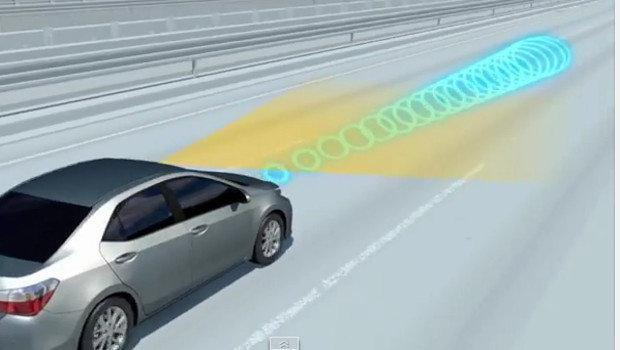
\includegraphics[width=300px, scale=1]{figuras/sinal_componentes}
    \caption{Revista Quatro Rodas}
  \label{fig:sinal_componentes}
  \end{figure}

\item \textbf{Custo}

  No RAV4 o Safety Sense (TSS) será um opcional. Logo, o comprador desejar um
  veículo que ofereça maior segurança, terá que pagar US\$ 30,00 a mais. No
  Lexus,  Lexus Safety System + (LSS+), o valor pago a mais será de US\$
  500,00.  \cite{1comper}

\item \textbf{Sistema Volvo}

Controle Ativo de Proximidade (ACC), sendo seu nome original Active Cruise
Control, é utilizado pela fabricante de veículos VOLVO para evitar colisões
entre veículos que trafegam na mesma direção e sentido.

\begin{figure}[h]
  \centering
  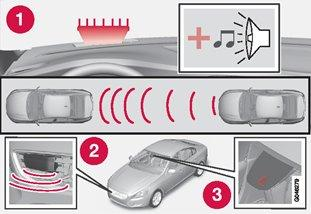
\includegraphics[width=300px, scale=1]{figuras/esquematico_volvo}
  \caption{Visão geral da função \cite{8comper}}
\label{fig:esquematico_volvo}
\end{figure}

1-Sinal de alerta audiovisual em caso de risco de colisão.

2-Sensor do radar;

3- Sensor da camera.

\item \textbf{ESPECIFICAÇÕES DO SENSOR E FUNCIONAMENTO}

Especificações gerais em um primeiro momento:

\begin{itemize}
  \item Faixa de medição de 0,5 m até 200 m;
  \item Possui alinhamento através de ondas eletromagnéticas com angulo de varredura de 12º;
  \item Parâmetros livremente programáveis;
\end{itemize}

O Aviso de colisão com Sistema automático de freio executa três etapas na seguinte ordem:

1. Aviso de colisão

2. Auxílio de frenagem

3. Frenagem automática

O Sistema anti colisão e o cidade segura se complementam.

1 – Aviso de Colisão

Primeiramente, o motorista é avisado sobre uma colisão potencialmente iminente.
[8] Se há risco de colisão com um pedestre, ciclista ou um veículo, então o
motorista é atraído com um sinal de alerta vermelho (8) e um sinal acústico. \cite{8comper}

2 – Auxílio de frenagem

Se o risco de colisão aumentou depois do aviso anti colisão, então o auxílio de
frenagem é ativado. Isto significa que o sistema de freio é ativado para uma
rápida frenagem aplicando levemente os freios, o que pode parecer com um leve
solavanco. Se o pedal de freio é pressionado rapidamente então a função que
freia totalmente o carro é acionada. Existe o auxilio também, caso o sistema
entenda que o freio do condutor nao foi suficiente. \cite{8comper}

3 – Frenagem automática

A frenagem automática é a última a ser ativada. Se nesta situação o motorista
ainda não começou a tomar uma ação evasiva e o risco de colisão é iminente,
então a frenagem automática é implementada – isto ocorre independentemente se
o motorista aciona o freio ou não. Em seguida ocorre a freada com a frenagem
completa para reduzir a velocidade colisão, ou com frenagem limitada se for
suficiente para evitar a colisão. Para os ciclistas, o aviso e a intervenção
com a frenagem completa podem vir simultaneamente ou tarde demais. \cite{8comper}

Observações: O sistema de aviso anti colisão não se aplica a todas as
situações de condução ou de trânsito, condições de tempo ou de estrada.
O sistema anti colisão não funciona se há veículos, ciclistas ou animais
em direções opostas.

A função de aviso anti colisão só é ativada se há um alto risco de colisão.
E avisos e intervenções de frenagem para pedestres e ciclistas são desativadas
se o veículo estiver com uma velocidade superior a 80 km/h; tal como não
funcionam em túneis e quando está escuro (mesmo se os faróis estiverem ligados).

O sistema pode frear o carro ou diminuir a velocidade se houver risco de colisão,
mas para assegurar o funcionamento é necessário que o motorista pressione o pedal
do freio e também afirma que o motorista nunca deve esperar pelo aviso de colisão
e sempre seguir as leis de trânsito e manter uma distância segura do veículo da
frente. \cite{8comper}

O sistema anti colisão tem uma restrição sobre o alcance, ele só consegue detectar
carros e objetos se estiverem em uma distância máxima de 150 metros. \cite{9comper}


\item \textbf{FREQUÊNCIA ENVOLDA}

A ZF TRW, empresa desenvolvedora desse tipo de sistema utiliza uma frequência de
24GHz ISM.

Já a BOSH produz este sensor utilizando a faixa entre 76-77 GHz,
isso representa uma varredura de até 160 m. A figura \ref{fig:bosh} mostra o
sensor desenvolvido pela BOSH.

\begin{figure}[h]
  \centering
  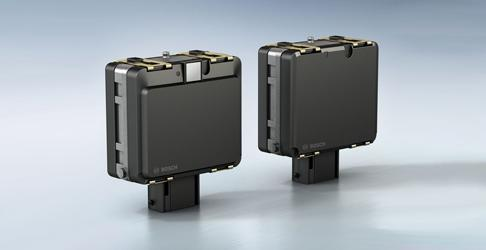
\includegraphics[width=300px, scale=1]{figuras/bosh}
  \caption{BOSH - Mid-range radar sensor.}
\label{fig:bosh}
\end{figure}
\end{enumerate}
